\subsection {Программная платформа и язык программирования}
Для решения поставленной задачи необходимо использовать функциональную, эффективную и удобную платформу для разработки. В качестве такой платформы была выбрана среда разработки Qt Creator.
Qt - это кросс-платформенная библиотека C++ классов для создания графических пользовательских интерфейсов (GUI) от фирмы Digia. Эта библиотека полностью объектно-ориентированная, что обеспечивает лёгкое расширение возможностей и создание новых компонентов. Ко всему прочему, она поддерживает огромнейшее количество платформ.

Qt позволяет запускать написанное с его помощью ПО в большинстве современных операционных систем путём простой компиляции программы для каждой ОС без изменения исходного кода. Включает в себя все основные классы, которые могут потребоваться при разработке прикладного программного обеспечения, начиная от элементов графического интерфейса и заканчивая классами для работы с изображениями, видео и мультипоточными приложениями. Qt является полностью объектно-ориентированным, легко расширяемым и поддерживающим технику компонентного программирования.

Список использованных классов фреймворка Qt:
\begin{itemize}
\item QDebug;
\item QDir;
\item QFile;
\item QTextStream;
\item QSrting;
\item *QImage;
\item QTime.
\end{itemize}

Класс QDebug обеспечивает выходной поток для отладочной информации.

Класс QDir обеспечивает доступ к структуре каталогов и их содержимого.

Класс QFile предоставляет интерфейс для чтения и записи файлов.

Класс QTextStream предоставляет удобный интерфейс для чтения и записи текста.

Класс QString обеспечивает строку символов Unicode.

Класс QImage предоставляет аппаратно-независимую работу с изображениями, даёт прямой доступ к данным каждого пикселя, и может быть использован в качестве устройства рисования. На ранних стадиях создание ПО это класс использовался в качестве основного инструмента для работы с изображениями, но впоследствии при переходе на основные модули библиотеки DV стал использовался объект Data2D, и методы работы с ними.

Класс QTime обеспечивает функции таймера. В проекте используется для оценки быстродействия разрабатываемого модуля при разных входных параметрах~\cite{qt}.

Для совместимости с библиотекой DV, решено использовать систему сборки CMake, взамен QMake. CMake широко используется с Qt.
Список классов и методов библиотеки DV используемых в проекте:
\begin{itemize}
\item Data2D;
\item Matx22d;
\item Vec2d;
\item VF2d.
\end{itemize}

Список стандартных библиотек используемых в проекте:

\begin{itemize}
\item getopt.h;
\item iostream;
\item math.h;
\item stdlib.h;
\item vector.
\end{itemize}

getopt библиотечная функция, специально разработанная для того чтобы облегчить обработку входных команд. 

iostream заголовочный файл с классами, функциями и переменными для организации ввода-вывода в языке программирования C++. Он включён в стандартную библиотеку C++. Название образовано от Input/Output Stream (``поток ввода-вывода'').

math.h — заголовочный файл стандартной библиотеки языка программирования С, разработанный для выполнения простых математических операций.

stdlib.h — заголовочный файл стандартной библиотеки языка Си, который содержит в себе функции, занимающиеся выделением памяти, контроль процесса выполнения программы, преобразования типов и другие.

vector.h — это замена стандартному динамическому массиву, память для которого выделяется вручную, с помощью оператора new.
\subsubsection {Использование системы контроля версий}
Система контроля версий (СКВ) — это система, регистрирующая изменения в одном или нескольких файлах с тем, чтобы в дальнейшем была возможность вернуться к определённым старым версиям этих файлов.

Для разработки программного комплекса решено использовать Git.

Git  — распределённая система управления версиями файлов. Проект был создан Линусом Торвальдсом для управления разработкой ядра Linux, как противоположность системе управления версиями Subversion (также известная как «SVN») \cite{progit}.

Преимущества использования системы версий, очевидны:
\begin{itemize}
\item возможность возвращать к прежнему состоянию отдельные файлы или весь проект;
%\item возможность создавать свои ветки, не мешая при этом другим разработчикам;
\item возможность удалённой работы с текстами программ;
\item доступ к последним изменениям в коде, т.к. всё хранятся на сервере github.com;
\item тексты программ открыты, доступ к ним можно получить доступ в интернет;
%\item удобство работы с tex документами;
\item просматривать происходящие со временем изменения.
\end{itemize}

Основные постулаты работы в системе Git:
\begin{itemize}
\item каждая задача решается в своей ветке;
\item сохраняем изменения сразу, как что-то получили осмысленное;
%\item в master мержится не разработчиком, а вторым человеком, который производит вычитку и тестирование изменения;
\item все сохранённые изменения должны быть осмысленно подписаны/прокомментированы.
\end{itemize}
\begin{figure}[ht]
\center{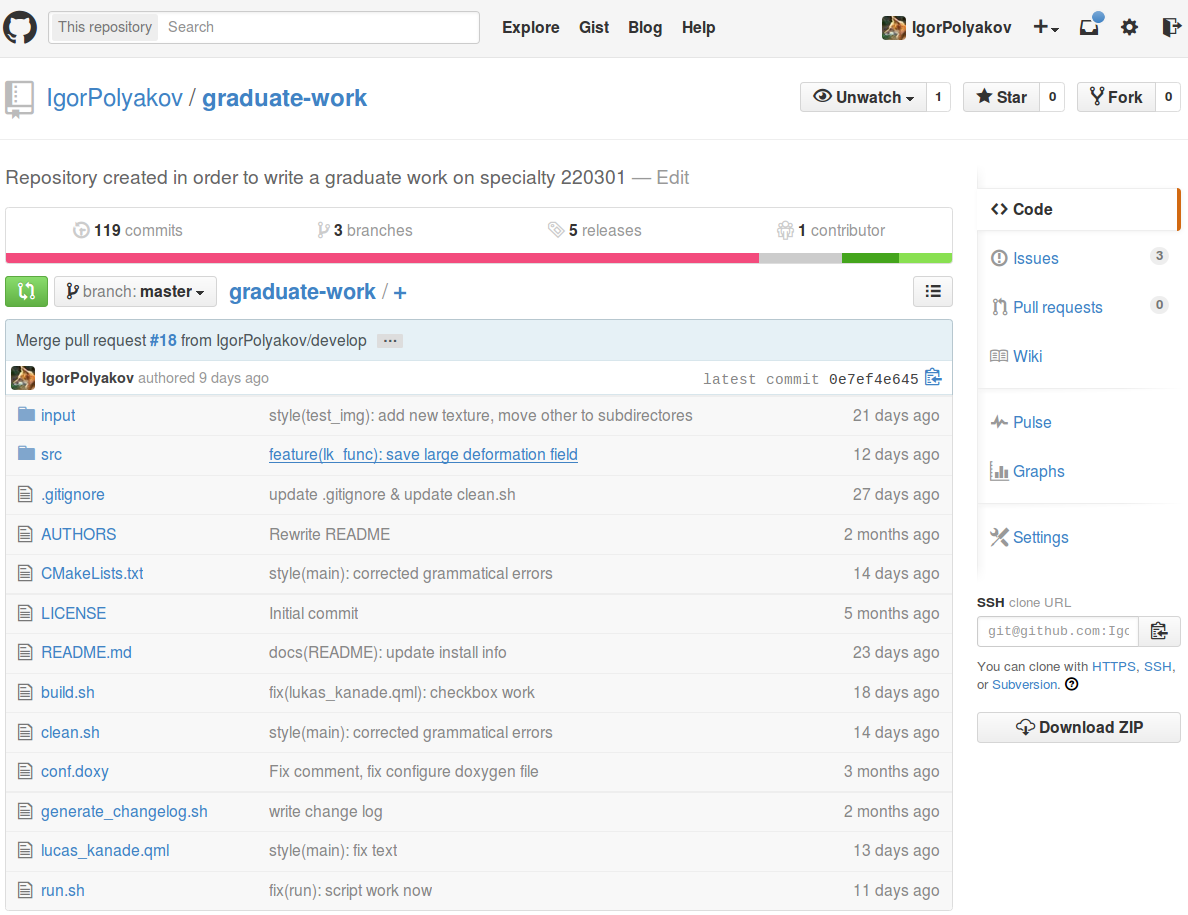
\includegraphics[width=0.9\linewidth]{github}}
\caption{Тексты программ в репозитории github}
\label{pic:github}
\end{figure}

Для работы над проектом был использован репозиторий на сервере github.com. Слепок последних изменений из репозитория можно взять по адресу: git clone git@github.com:IgorPolyakov/graduate-work.git


\subsection{Структурно функциональная схема программного обеспечения}%, в состав которого входит разрабатываемый программный модуль с четкой формулировкой решаемых им задач}

Программное обеспечение состоит из нескольких блоков, представленных на рисунке \ref{pic:shema_PO}.

\begin{itemize}
\item ПО для оценки деформации ``Deformation Analysis''
\item Форма для ввода входных параметров ``strain\_calculate.qml''
\item ПО для расчёта деформации твердого тела ``lucas\_kanade''
\end{itemize}

Программа ``Deformation Analysis'' разрабатывалась сотрудниками ИФПМ и служит средством для запуска и отображения выходных результатов. Форма ``strain\_calculate.qml'' является более удобным способом запуска основного приложения. 

\begin{figure}[ht]
\center{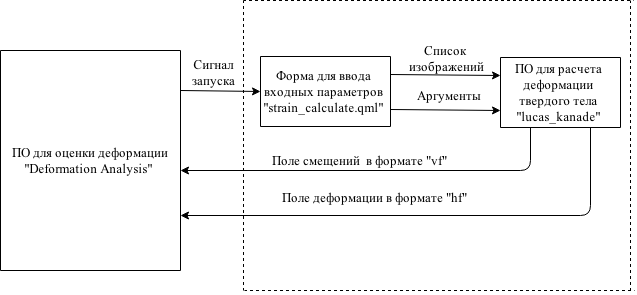
\includegraphics[width=0.8\linewidth]{shema_PO}}
\caption{Структура разработанного ПО}
\label{pic:shema_PO}
\end{figure}

\begin{figure}[ht]
\center{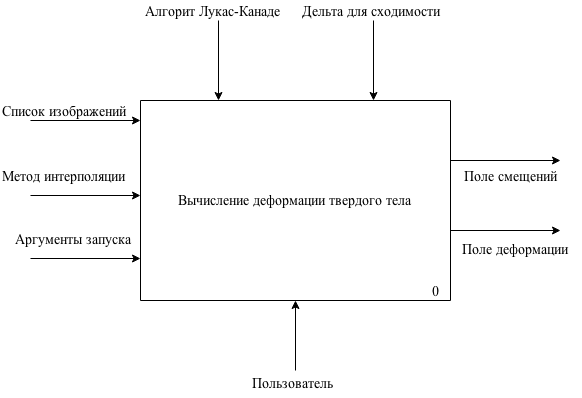
\includegraphics[width=0.8\linewidth]{idef0}}
\caption{Функциональная схема}
\label{pic:idef0}
\end{figure}

\begin{enumerate}
\item  укрупненная структурно функциональная схема программного обеспечения, в составе которого работает модуль. Разрабатываемый модуль должен быть визуально выделен на общей схеме (обведён штриховой рамкой, обозначен другим цветом и т.д.);
\item  структурно функциональная схема разрабатываемого программного модуля с обозначением входящих в него функциональных элементов и связей между ними. В связях надлежит доступными средствами выделить различные виды информационных потоков: символьные и кодовые массивы, бинарные сигналы индикации и управления, событийную информацию;
\item  основные математические соотношения в виде формул и выражений (при разработке вычислительных программ не более, чем 1 плакат формата А1);
\item  блок схема алгоритма работы модуля с достаточной степенью детализации (при наличии в разработке оригинальных и неочевидных алгоритмических решений);
\item  изображения экранных форм в различных режимах работы программы(при разработке интерфейсных модулей);
\item  материал, иллюстрирующий работу программы на тестовом или реальном примере, с использованием графиков, таблиц и пр.
\end{enumerate}

\subsection{Сведения о платформе реализации с указанием основных функций операционной системы, необходимых для работы модуля}
Для корректной работы разрабатываемого программного комплекса, компьютер должен отвечать следующим требованиям:
\subsubsection {Минимальные требования к аппаратному обеспечению}
Минимальные системные требования для операционной системы Linux Debian 8~\cite{debian_8}:

\begin{itemize}
\item процессор 1ГГц Pentium 4;
\item оперативная память 512 Мб;
\item место на жёстком диске -- 9 Гб.
\end{itemize}

Минимальные системные требования для операционной системы Microsoft Windows 7~\cite{windows_7}:

\begin{itemize}
\item процессор 32-разрядный или 64-разрядный 1 ГГц;
\item оперативная память 1 Гб для 32-разрядной системы или 2 Гб для 64-разрядной системы;
\item 16 Гб для 32-разрядной системы или 20 Гб для 64-разрядной системы пространства на жестком диске;
\item графическое устройство DirectX 9 с драйвером WDDM 1.0.

\end{itemize}

\subsubsection {Минимальные требования к программному обеспечению}
Для корректной работы разрабатываемого программного комплекса на компьютере должны быть установлены:
\begin{itemize}
\item Qt5 или Qt4;
\item CMake не ниже 2.8;
\item HDF5 не ниже 1.8.
\end{itemize}

\subsection {Выбор формата выходных файлов}
Для вывода результата был выбран формат файла HDF5. 

Hierarchical Data Format, HDF (Иерархический формат данных) — название формата файлов, разработанного для хранения большого количества цифровой информации.

HDF5 — современная версия формата содержит иерархию из двух основных типов объектов:
HDF-Structure-Example
\begin{enumerate}
\item Datasets — наборы данных, многомерные массивы объектов одного типа
\item Groups — группы, являются контейнерами для наборов данных и других групп
\end{enumerate}
    
Содержимое файлов HDF5 организовано подобно иерархической файловой системе, и для доступа к данным применяются пути, сходные с POSIX-синтаксисом, например, /path/to/resource. Метаданные хранятся в виде набора именованных атрибутов объектов.\cite{hdf5}
\begin{figure}
\centering
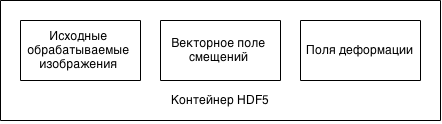
\includegraphics[width=0.7\linewidth]{images/structHDF5}
\caption{Структура HDF5 файла}
\label{fig:structHDF5}
\end{figure}

Структура сохранения результатов работы представлена на рисунке \ref{fig:structHDF5}

Под блоком исходные обрабатываемые изображения подразумевается входная пара изображений(левая, правая) в форматах png, bmp, jpg, tiff и др. В выходном файле они представлены двумя слоями: ``left'' и ``right''. Они необходимы для удобства просмотра в программе Defomation-Analysis. Программа Defomation-Analysis умеет выводить отдельные слои и накладывать их друг на друга.

Блок векторное поле смешений является бинарным файлом, формата ``vf''. Слой содержит информацию о размерах исходного изображения, координаты векторов смещений и векторы в формате double (формула \ref{eq:lucas}).

Блок поля деформации также является бинарным файлом и содержит слои деформации:
\begin{enumerate}
\item $\varepsilon_{xx}$ - продольная (формула \ref{eq:e_xx});
\item $\varepsilon_{yy}$ - поперечная (формула \ref{eq:e_yy});
\item $\varepsilon_{xy}$ - сдвиговая (формула \ref{eq:e_xy});
\item $w_{i}$ - поворотная (формула \ref{eq:w_z});
\item $\gamma_z$ - интенсивность деформации сдвига (формула \ref{eq:gamma_i}).
\end{enumerate}

\subsection{Документирование ПО}
Для облегчения написания документации к текстам программ, можно воспользоваться генератором документации. Так как у автора работы есть опыт использования системы Doxygen, то она и будет использована.

На вход такого генератора поступает специальным образом комментированный текст программы, а иногда и другие компоненты программы, а на выходе создаётся готовая документация для распространения и использования.

Используемая система Doxygen как раз и выполняет эту задачу: она позволяет генерировать на основе исходного кода, содержащего комментарии специального вида, красивую и удобную документацию, содержащую в себе ссылки, диаграммы классов, вызовов и т.п. в различных форматах: HTML, LaTeX, CHM, RTF, PostScript, PDF, man-страницы.

Документация собранная системой Doxygen представления в приложении.
\subsection{Блок схему оригинальных, разработанных автором, алгоритмов работы основных, по мнению автора, программных модулей}
Основной алгоритм работы представлен на рисунке \ref{fig:lucas_kanade_alg}. Для удобства, крупное блоки вынесены в отдельные блок-схемы и представлены на рисунках \ref{fig:calc_pyr} и т.д. 
\begin{figure}
\center{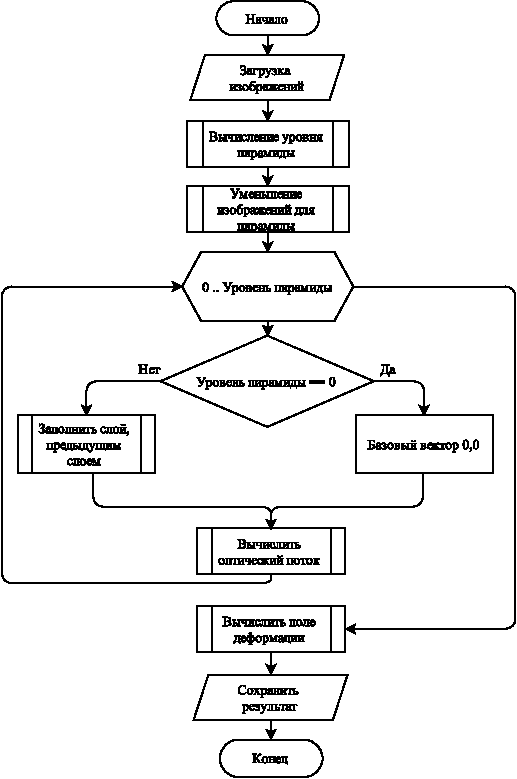
\includegraphics[width=0.7\linewidth]{images/lucas_kanade_alg}}
\caption{Общий алгоритм работы}
\label{fig:lucas_kanade_alg}
\end{figure}

\begin{figure}
\center{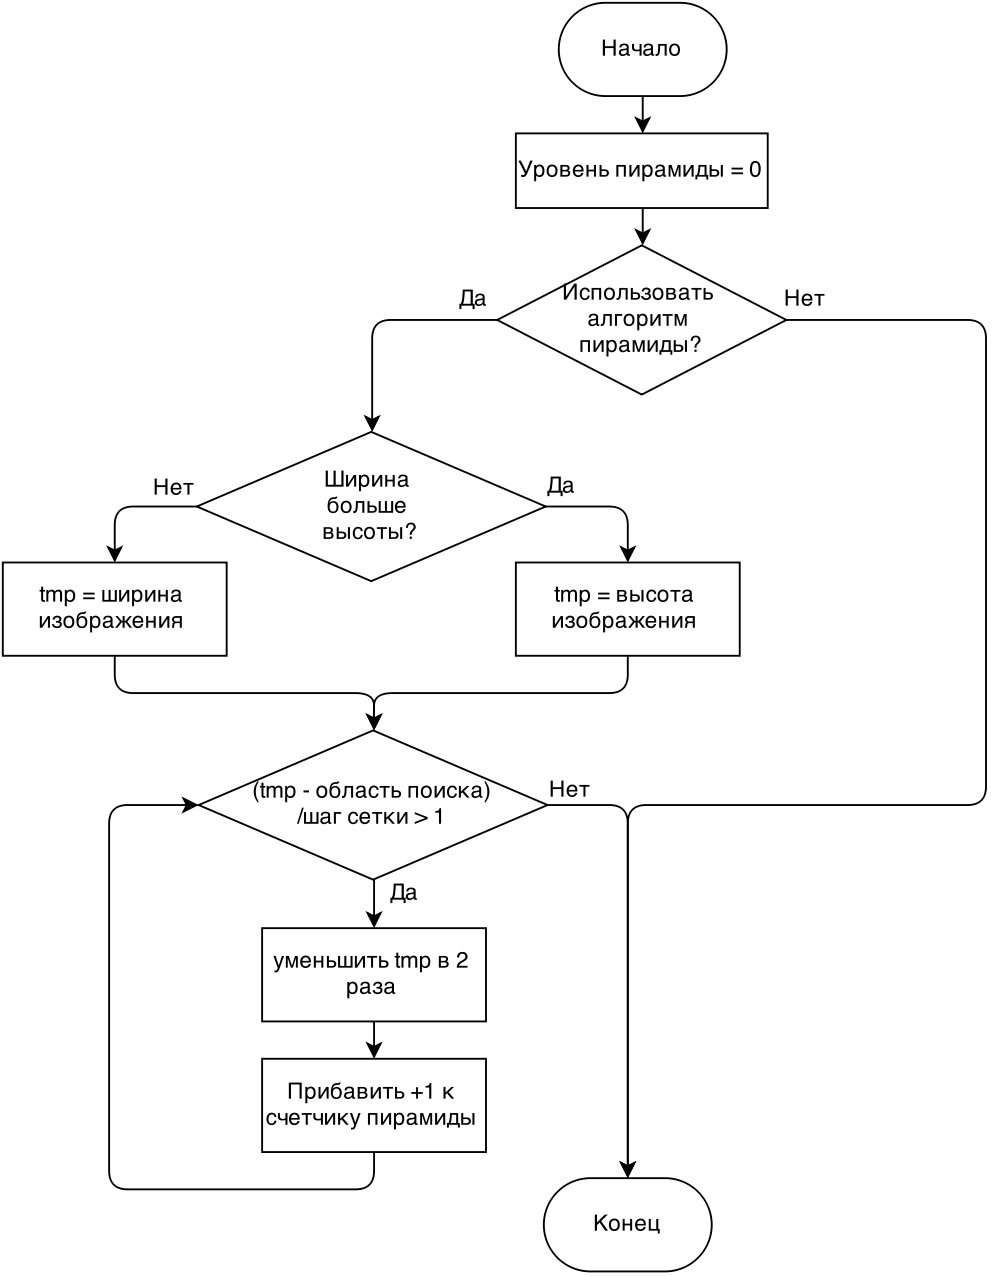
\includegraphics[width=0.7\linewidth]{images/calc_pyr}}
\caption{Адгоритм вычисления уровня пирамиды}
\label{fig:calc_pyr}
\end{figure}

\subsection {Интерфейс разрабатываемого программного обеспечения}
\subsubsection{Описание консольного интерфейса программы}% (выбор цветовой палитры экранных форм, расположение элементов управления на них, использование «горячих» клавиш  акселераторов, выпадающих меню и пр.)}
Интерфейс программы представлен в двух реализациях.
Первый — консольная программа в стиле классического Unix. Интерфейс командной строки более гибкий, позволяет выставить необходимые опции/флаги и запустить программу. Особенности в сравнении с графическим интерфейсом:
\begin{itemize}
\item интерфейс командной строки позволяет писать скрипты для автоматизации запуска и тестирования с различными входными параметрами, что средствами графического интерфейса гораздо сложнее;
\item большая функциональность;
\item некая сложность при использовании неопытным пользователям;
\item невозможность просмотра выходных результатов.
\end{itemize}

\begin{figure}[ht]
\center{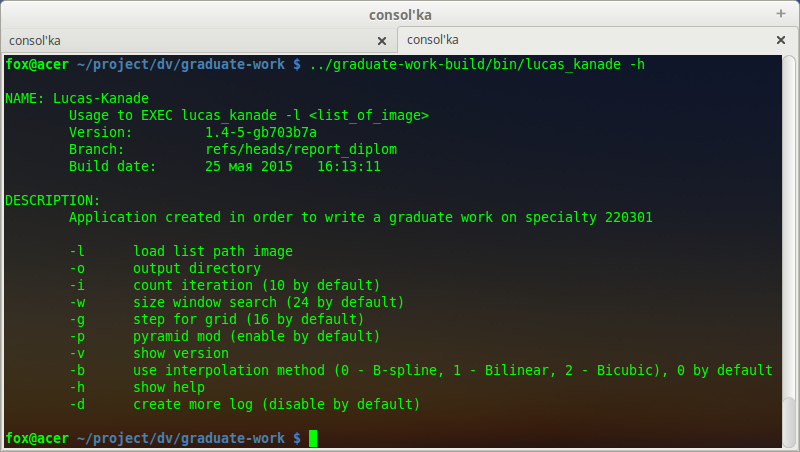
\includegraphics[width=0.8\linewidth]{consol_screen}}
\caption{Пример консольного интерфейса в среде Linux}
\label{pic:con_scr}
\end{figure}

Перечень команд для запуска:
\begin{itemize}
\item l — список изображений для обработки;
\item o — директория для выходных результатов;
\item i — число уточнений при поиске смещённой части (по умолчанию равна 10);
\item w — радиус окна поиска (по умолчанию равна 24);
\item g — шаг между векторами оптического потока(по умолчанию равна 16);
\item p — применить метод пирамиды(по умолчанию опция включена);
\item v — показать версию программного обеспечения;
\item b — использование метода интерполяции(0 — Б-сплайн, 1 — Билинейная, 2 — Бикубическая), по умолчанию 0;
\item h — показать краткую справку;
\item d — генерировать подробный лог файл(по умолчанию опция выключена).
\end{itemize}
\subsubsection{Описание графического интерфейса программы}
Второй графический — более удобный для неопытного пользователя. Общий вид ПО приведен на рисунке \ref{pic:gui_scr}. 
\begin{figure}[ht]
\center{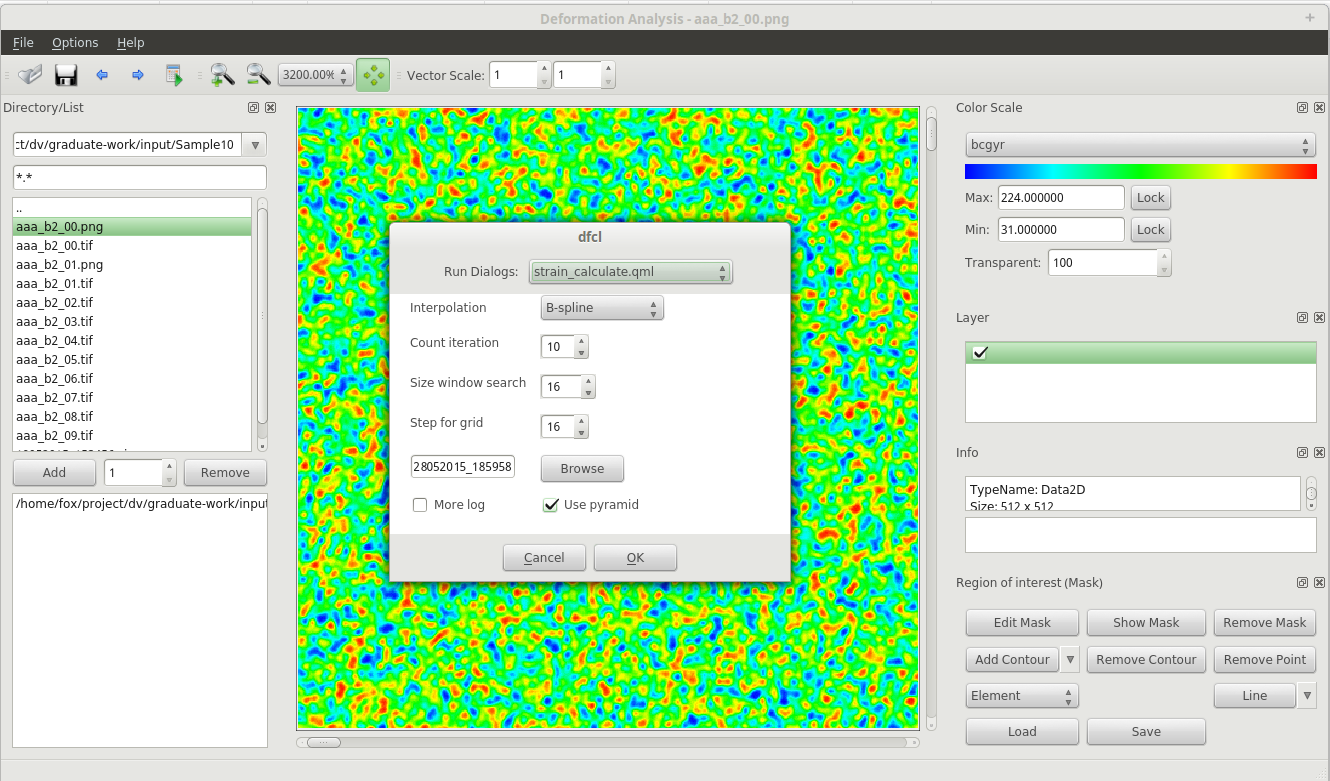
\includegraphics[width=0.95\linewidth]{gui_screen}}
\caption{Пример графического интерфейса}
\label{pic:gui_scr}
\end{figure}
Главное окно приложения включает в себя:
\begin{itemize}
\item окно просмотра документа;
\item список файлов в директории;
\item главное меню;
\item панели инструментов;
\item список файлов добавленных на обработку.
\end{itemize}
Форма запуска приложения, содержит большинство описанных ранее функций:
\begin{itemize}
\item метод интерполяции
\item число уточнений при поиске смещённой части (задаётся в диапазоне от 10 до 100);
\item радиус окна поиска (по умолчанию равна 24);
\item шаг между векторами оптического потока(по умолчанию равна 16);
\item директория для выходных результатов;
\item режим логов;
\item режим пирамиды.
\end{itemize}